\label{sec:sim_options}
The goal of this specialization project is to build a simulator which is applicable to the case of the Plan Sea project. There are five elements that need to be simulated for this to be considered a success. 
\begin{itemize}
\item Surface vessel
\item Subsurface vessel
\item Connecting wire
\item Weather impacts
\item Control system
\end{itemize}

Of these points, all of them can be simulated fairly simply with purely  analytical methods except for the connecting tether. Wire physics are a notoriously difficult thing to simulate because they are not rigid bodies. They have strength in tension but not in compression, leading to a discontinuous behaviour. You can't push a rope, or wire in this case. 

There are two main paths to take with regards to making the simulation. I could make everything from scratch from first principles or I could use an already existing simulation framework and build something on top of that. Both solutions have positives and negatives. 

Creating a system from scratch would be an interesting challenge. It would also give me exactly the results I'd want with very little overhead, assuming that my own programming skills are up to the task. The bespoke, home-made simulator also wouldn't have any associated licensing costs. On the other hand, to create a simulator which includes buoyancy, fluid dynamics, wire physics, handles a coupled system and also has some form of graphical interface/readout for the user is a large task to undertake. 

Using a commercially available system also has a fair few benefits. I would have a mostly ready-made framework which I can just configure the simulation at hand within. Changing out parameters and variables would also be very simple, as it's essentially the same as the original configuration. I believe also that the results from a commercial solution would be more reliable than my own attempt. It is reasonable to assume that an industrially used simulation solution made by a team of physicists, computer engineers and other specialists is fairly accurate with regards to its results. The same cannot be said for a cobbled-together solution made by one student in roughly 6 months. Commercially available solutions are not all perfect however. There are licensing costs associated with many simulation frameworks. Some having enormous costs for the scale of a student project. There is also likely more overhead with a commercially available solution due to them being as wide in their application as possible, to allow for as many customer types as possible. This can make the commercially available solution slower or less responsive. 

After considering the points above for both commercially available and personally crafted simulation frameworks, I decided that using a ready-made solution would be better. This was especially decided because of the time constraints of this project. My goal is to have a working simulation that can be used to provide information, the goal is not to make a simulator. If I was to make it myself, the project would quickly turn into "make a simulator" rather than "make a simulation", simply because of the scale of the undertaking. 

\section{AGX}
After considering multiple simulation options and on the advice of a professor, I landed on using AGX, made by Algoryx, as a simulation framework. AGX has a solid wire simulation package, a hydrodynamic simulation package, and allows for scripting and setup using both Python and C++. It has interfaces towards both Unreal Engine and the Unity engine for further graphical display of the results. In addition, AGX has interfaces for ROS2 which I will get into in \cref{sec:ros}. 

My implementation of AGX is based on Python as that's the language I'm most familiar with. I am aware of Python's inferiority to a C++ based approach in terms of speed and efficiency in resource use, but the time investment required for me to get to an acceptable level of C++ proficiency was not worth it for this project.



\subsection{Limitations of AGX}
By using a ready-made simulation platform I am able to quickly implement a simulation without needing to worry about the mathematical models that exist behind the simulation. This allows me to focus on achieving results, although it also necessitates a degree of trust in the simulation. I am able to verify whether the simulator acts as expected or not, but changing the governing equations is not necessarily something I am able to do. 

Another limitation of AGX is that it's a licensed software. This means that in order to apply and use the findings of this report, the software needs to be acquired. This is a limitation for further research, and ideally the findings should be based on open and available software or arrived at from first principles. 

\section{Description of the simulation setup}
The simulation starts with defining a water volume. This is done using AGX built-in functions. Currently the volume is 100m along the sides and 50m deep, though this is arbitrary. I've implemented one "water controller" which is the object that handles wave, current and wind forces. Currently this controller is completely still and there is no force inputs, but it is implemented so that adding weather forces is simple for later iterations. In AGX, each element in a simulation has to be individually added to that simulation. Once both the water volume and the water controller have been added to the active simulation, the vessels are made.

The surface vessel and the ROV are both implemented as children of a parent class for general vessels. I've done this for ease of expansion later. The ROV is just a simple box with a given density and size. The ROV's size I've taken from BlueROV's websites\cite{noauthor_bluerov2_nodate}, as an example of the size of ROV we will be working with in this project, though as mentioned it's just implemented as a box. The University does currently have a BlueROV that is intended to be used for the initial steps of the Plan Sea project, as well as for my master's thesis which will be based on this work, that is why I've chosen to use their dimensions. The exact dimensions are \(0.45m \times 0.575m \times 0.254m\) for a total volume of \(0.0654m^3\). If a more accurate shape for the ROV is desired, it is possible to implement it similarly to the surface vessel, but since this project is mostly a first-order approximation of the problem, I believe a simple box is sufficient. The ROV's density I have wildly exaggerated and arbitrarily chosen to be \(2000\frac{kg}{m^3}\). This is an absurd exaggeration and should be replaced with more relevant data later, but for a proof of concept it will work fine. This gives a total mass of the ROV of 131kg. The surface vessel's shape is defined by a wireframe stored in an \texttt{.obj} file I've made that approximates the shape of the hull, while its density I've approximated from the density of the carbon-fiber sandwich board used to \(600\frac{kg}{m^3}\). The simulation software has provided a mass calculation for the vessel to approximately 2300kg. This gives the ratio of mass between the two vessels of roughly 5\%, which is far more than an assumed real-world estimation of less than 1\%. This will skew the results to favour the impacts of the ROV. 

\begin{figure}
	\centering
	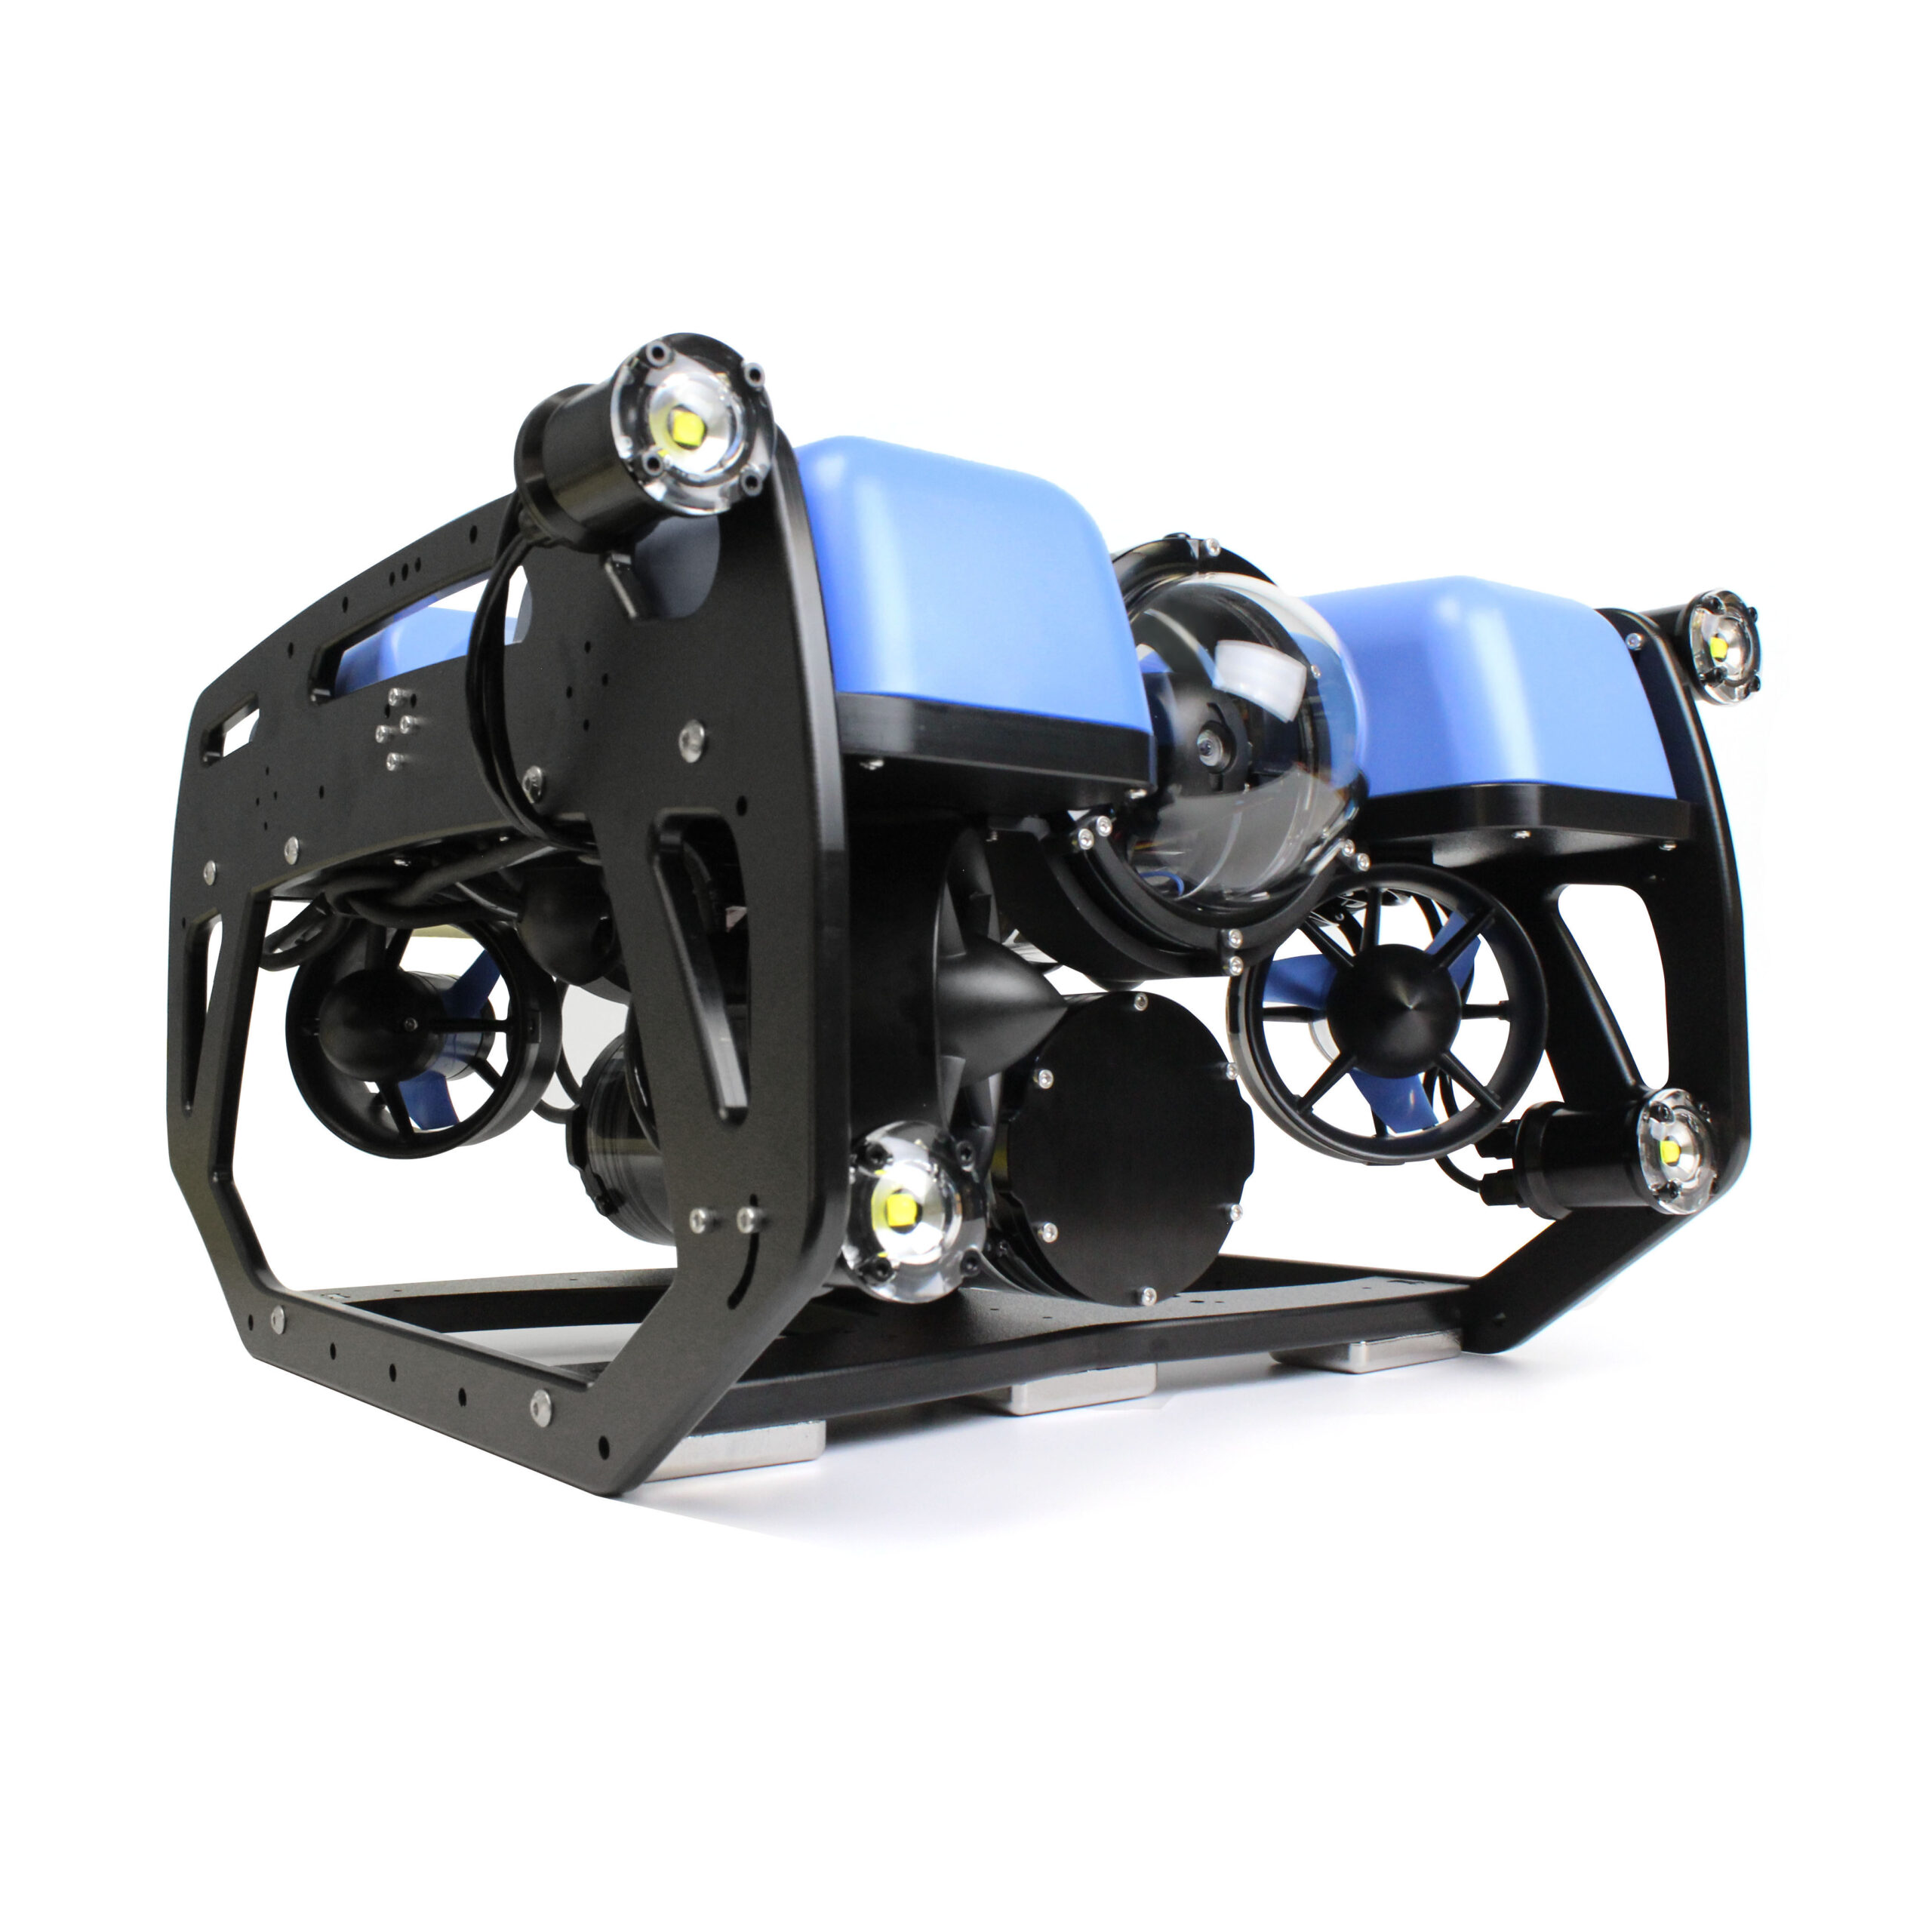
\includegraphics[width=0.5\textwidth]{bluerov}
	\caption{Illustration image of the BlueROV2 used as a basis for the ROV in this project. Credit: BlueRobotics}
	\label{fig:bluerov}
\end{figure}

In addition to a class which handles the shape and properties of the surface vessel, I have made a class that handles controlling the vessels. The controller is just a simple implementation of a PD controller. The controller checks the position of the vessel on each timestep and calculates an error. The error is then controlled using the PD controller and a response is found. The response is clamped within a given authority limit. I've done this because realistically, the control authority of the system is going to be limited because of the physical capabilities of the thursters. I've estimated the authority for right now, but it should be changed later when the real command authority is found. 

Currently, the way the controller is acting on the vessel is by simply applying a force in a given direction on the CoG of the vessel. For the surface vessel, any force and error given in Z-direction is zeroed as the surface vessel will not be able to cancel its own heave in waves. This can be changed later and the Z-direction error/control can be implemented as heave-compensation for the ROV. This isn't implemented yet though. I've also implemented a simple proportional controller for heading control which works by adding a torque to the body it's controlling. In a future iteration, both the simplistic control and heading control could be implemented by splitting the force inputs from one single input at CoG to one input at the position of each thruster. Then yawing motion will also be applied with differential thrust and a yaw-term can be added to the controller. Whether the complications of simulating force inputs at the thruster locations are necessary is not clear yet. If we consider the ideal future implementation in a physical vessel, the controller designed now is only intended to give the total commands to the vessel. Thrust allocation and local control will be designed elsewhere and simply be a node in the ROS2 system that will be the final vessel. Either way, the option of making the simulation more true to life exists if it should be desirable. 

Finally, the wire which connects the ROV and the surface vessel is created. AGX has two similar wire-like simulation objects: Wires and Cables. According to the documentation, because torsion of the wire is irrelevant, we want to be able to winch the wire in and out to simulate lifting and lowering the ROV and we are working on long wires, the Wire module should be used. The way wires work in AGX is as a series of links connected to or passed through a series of nodes. For this implementation only two nodes are necessary, one connecting the wire to the surface vessel and one connecting it to the ROV. The Wire module of AGX allows for winches to be simulated as well, with given speeds, gearings, torques etc.. I have not implemented this currently due to time constraints. 

In addition to all the "necessary" elements, the simulation also has a manual controller for the vessels. It is possible to use the keyboard to give manual force inputs on the vessels. This uses the same framework for adding force as the controller does. I've done this as a way to debug and test the system a bit.

The final simulator can be seen on Github\cite{noauthor_fordypogmastersimulator_nodate}. The URL is \url{https://github.com/MagnusKjorseng/FordypOgMaster/tree/main/Simulator/V3}

\section{ROS2}
\label{sec:ros}
ROS2, short for Robot Operating System 2, is an easily expandable and configurable operating system used primarily for hobbyists and research in control and robotics. The main selling point of ROS2 is its node model where different parts of a control system can be placed in separate, segregated nodes with certain interfaces. Those nodes then either publish data to or subscribe to data from what ROS2 calls topics. This system grants a developer or team of developers flexibility with regards to changing out certain nodes while still allowing the larger system to work. I.e. experimenting and changing out single nodes, so long as the same topics are still used, is extremely simple. 

I was not able to implement ROS2 during this project. I believe this is because ROS2 is not designed to be used on Windows and requires a lot of workarounds which I was not able to figure out. This section is in the report more as a reference and a reminder for future iterations based on this report that ROS2 would make the project easily scalable and iterable. 

AGX has the ability to work with ROS2, having built in methods for both publishing and subscribing to topics. Applied to this project it would in theory allow for the control system to be built in ROS2 and connected to the simulator. The control system could then be tested and tuned in different simulated environments until satisfactory results are achieved. When the control system works as intended, it can then be disconnected from the simulator and connected to a physical implementation of the simulated environment which would allow for real-world testing. 

The end result of the process above would be two equivalent systems, one digital and one physical, which would allow for rapid prototyping in the digital space before quick deployment in physical space. 

